\chapter{Multi-Tasking}

\section{Task}
I task rappresentano le azioni da eseguite concorrentemente nel sistema. 

\begin{itemize}
	\item Dal \textbf{punto di vista del progettista}:
	\begin{itemize}
		\item sono dei moduli software che impegnano il microprocessore per un certo periodo;
		\item permettono di eseguire calcoli e/o azioni di I/O;
		\item possono essere sostituiti, alterati o modificati in base alle necessità.
	\end{itemize}
	\item Dal \textbf{punto di vista dell'utente} invece:
	\begin{itemize}
		\item  creano l'illusione di avere un unico sistema monolitico;
		\item  la semplice esistenza e quindi la loro gestione è trasparente all'utente.
	\end{itemize}
\end{itemize}


\subsection{Le espressioni Lambda in Wiring/C++11}
Una \textbf{Lambda expression} (\textit{lambda closure}) è una funzione anonima definita al momento della chiamata. 

Sintassi accettate dal compilatore di Arduino:
\begin{lstlisting}[language=C++]
[ capture-list ] ( params ) { body }
[ capture-list ] { body } 
\end{lstlisting}

\subsubsection{Caratteristiche}
\begin{itemize}
	\item La capture list è la lista di variabili che è possibile utilizzare oltre agli argomenti della funzione.
	\begin{itemize}
		\item Se si definisce [\&], tutte le variabili locali saranno passate per riferimento.
		\item Se non viene specificato niente, la lambda function non ha variabili come argomenti e viene indicata con [];
	\end{itemize}
	\item Il tipo di ritorno è void, a meno che non viene specificato diversamente;
	\item Il body della funzione che si trova tra parentesi graffe rappresenta le azioni che devono essere eseguite.
\end{itemize}

\subsubsection{Vantaggi}
\begin{itemize}
	\item programmazione più dichiarativa,
	\item modularizzazione,
	\item codice chiaro e semplice da leggere e mantenere,
\end{itemize}

\subsubsection{Contro}
Per utilizzare le lambda expression in questo progetto siamo stati costretti a rinunciare parzialmente all'\textit{information hiding} della programmazione O-O, in quanto non è stato possibile passare oggetti come parametro di chiusura. L'unico modo per passare gli oggetti e quindi i metodi all'interno di queste particolari funzioni è stato mettere tutto \texttt{public}

\subsection{Generalizzazione del funzionamento di un task}
\begin{figure}[!ht]
	\centering
	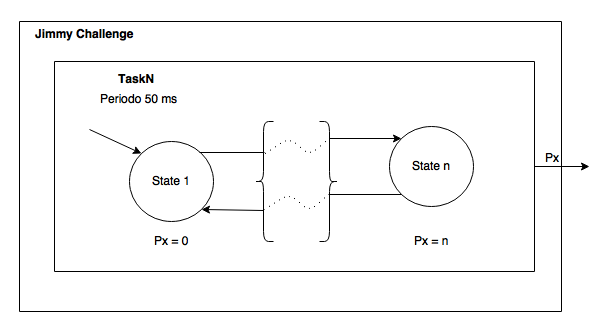
\includegraphics[scale=.60]{img/task_generic.png}
	\caption{Generalizzazione dei task}
\end{figure}

\subsubsection{Elenco dei Task sviluppati:}
\begin{enumerate}
	\item SonarTask
	\item ButtonTask
	\item BuzzerTask
	\item LedTask
	\item LedPwmTask
	\item LedRgbTask
\end{enumerate}

\subsection{SonarTask}
È il task più importante del progetto. Dal punto di vista funzionale serve a far interagire l'utente con il sistema.

\subsection{ButtonTask}
Questo task controlla se è avvenuta la pressione del \textit{button}.

\subsection{BuzzerTask}
Questo task controlla l'emissione dei suoni che devono essere emessi dal \textit{buzzer}

\subsection{LedTask}
Questo task controlla l'accensione e lo spegnimento del LED verde.

\subsection{LedPwmTask}
Questo task controlla modifica l'intensità del LED verde permettendone l'accensione o lo spegnimento istantaneo o temporizzato.

\subsection{LedRgbTask}


\section{Scheduler}




